\section{LEVEL 3 · Steekproef en representativiteit}

\begin{missie}
Missie: weet wanneer je een steekproef kan vertrouwen. (LPD 11)
\end{missie}

\begin{doel}
\textbf{DOEL} \quad Na dit level kan je:

☐ redenen geven waarom men met een \textbf{steekproef} werkt in plaats van met de volledige populatie;

☐ verklaren wat een \textbf{representatieve} steekproef is en waarom dat belangrijk is voor besluiten over de populatie;

☐ voorbeelden van \textbf{vertekende steekproeven} (selectiebias) herkennen en verklaren;

☐ het verschil uitleggen tussen een \textbf{steekproefgrootheid} en een \textbf{populatieparameter}.
\end{doel}

\subsection*{Theorie 3.1 · Waarom een steekproef?}

\begin{theorie}
Meestal willen we iets weten over een \textbf{populatie} (bijvoorbeeld alle jongeren in Vlaanderen), maar we onderzoeken enkel een \textbf{steekproef}. Dat doen we omdat:

\begin{itemize}
\item het \textbf{onmogelijk} is om iedereen te bereiken (te veel mensen, niet iedereen bereikbaar);
\item een volledig onderzoek te veel \textbf{tijd} kost (de uitslag moet snel beschikbaar zijn);
\item een volledig onderzoek te veel \textbf{geld} kost;
\item het onderzoek soms het product vernietigt (een lamp die je test tot ze stuk gaat, kan je daarna niet meer verkopen).
\end{itemize}

Op basis van de steekproef formuleren we een \textbf{statistisch besluit} over de populatie. Dat besluit is enkel betrouwbaar als de steekproef \emph{representatief} is.
\end{theorie}

\subsection*{Theorie 3.2 · Representatief of vertekend?}

\begin{theorie}
Een steekproef is \textbf{representatief} als ze een verkleinde, getrouwe afspiegeling is van de populatie: de kenmerken komen in de steekproef in dezelfde verhoudingen voor als in de populatie.

Een steekproef is \textbf{vertekend} (er is \textbf{selectiebias}) als bepaalde groepen systematisch te vaak of te weinig in de steekproef zitten.

Een steekproef wordt meestal representatief door \textbf{aselecte (toevallige) trekking}: elke eenheid van de populatie heeft evenveel kans om gekozen te worden, bijvoorbeeld door te loten uit een volledige lijst.
\end{theorie}

\begin{center}
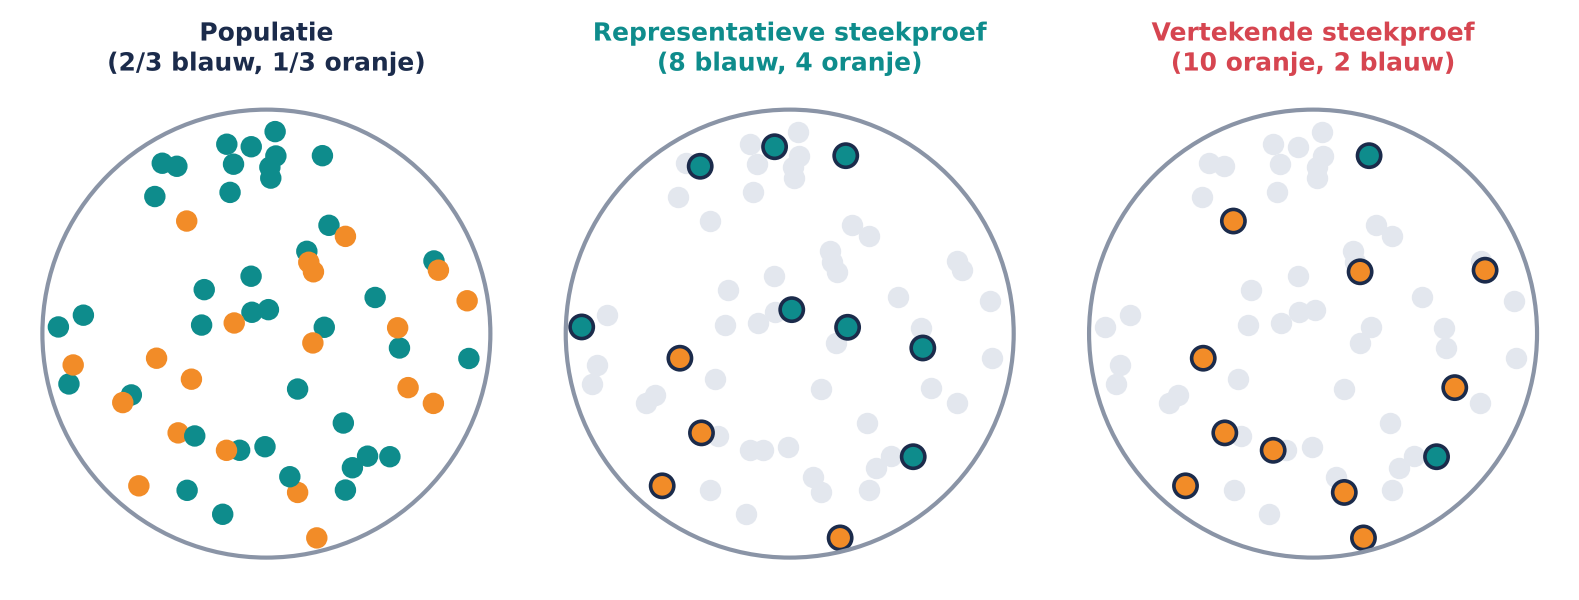
\includegraphics[width=0.95\textwidth]{figuren/l3_steekproef.png}
\end{center}

\textbf{Veelvoorkomende vormen van selectiebias:}

\breedtes{30/70}
\begin{tabular}{ll}
\hline
Vorm & Voorbeeld \\
\hline
\textbf{Zelfselectie} (vrijwillige respons) & Een online poll: vooral mensen met een sterke mening klikken. \\
\textbf{Gemakssteekproef} & Je ondervraagt alleen je vrienden of de mensen die toevallig in de buurt zijn. \\
\textbf{Onderdekking} & Een telefoonenquête enkel via vaste lijn: je mist wie geen vaste lijn heeft. \\
\textbf{Overlevers} & Een tevredenheidsenquête enkel bij wie de opleiding afmaakte: de afhakers ontbreken. \\
\textbf{Niet-respons} & Wie de vragenlijst niet invult, verschilt vaak van wie ze wel invult. \\
\hline
\end{tabular}

\begin{voorbeeld}
\textbf{Voorbeeld.} Een kinderopvang wil weten hoe tevreden ouders zijn en legt een vragenlijst op de infoavond. Op die avond komen vooral betrokken ouders. De ouders die minder betrokken of ontevreden zijn, ontbreken. Gevolg: de steekproef is vertekend en het besluit ‘90 \% is tevreden’ is niet betrouwbaar voor álle ouders.
\end{voorbeeld}

\begin{letop}
\textbf{LET OP} \quad Een \emph{grote} steekproef is niet automatisch een \emph{goede} steekproef. Een online poll met 10\,000 reacties blijft vertekend; een kleine, goed getrokken steekproef is vaak betrouwbaarder. Representativiteit gaat boven grootte, al zorgt een grotere representatieve steekproef wel voor een kleinere afwijking.
\end{letop}

\subsection*{Theorie 3.3 · Steekproefgrootheid of populatieparameter?}

\begin{theorie}
Een \textbf{populatieparameter} is een kengetal van de hele populatie en meestal onbekend. We \textbf{schatten} hem met een \textbf{steekproefgrootheid}.

\breedtes{34/33/33}
\begin{tabular}{lcc}
\hline
 & steekproef & populatie \\
\hline
omvang & $n$ & $N$ \\
gemiddelde & $\overline{x}$ & $\mu$ \\
variantie & $s^2$ & $\sigma^2$ \\
standaardafwijking & $s$ & $\sigma$ \\
\hline
\end{tabular}

Bij een representatieve steekproef is $\overline{x}$ niet systematisch groter of kleiner dan $\mu$. Toch zal $\overline{x}$ van steekproef tot steekproef wat verschillen: dat heet \textbf{steekproefvariabiliteit}. Hoe groter de (representatieve) steekproef, hoe kleiner de afwijking meestal is.
\end{theorie}

\subsection*{Aan de slag}

\subsubsection*{Oefening 3.1 \quad ★☆☆ \quad Invullen}

\textbf{Woordenlijst:} populatie – steekproef – representatief – selectiebias – parameter – vertekend.

Meestal is het onmogelijk of te duur om de volledige \gat{populatie} te onderzoeken. Daarom onderzoeken we een \gat{steekproef}. Die moet \gat{representatief} zijn: een getrouwe afspiegeling van de populatie. Als bepaalde groepen systematisch te weinig voorkomen, is er \gat{selectiebias} en is de steekproef \gat{vertekend}. Het gemiddelde van de populatie is een \gat{parameter}; die schatten we met het steekproefgemiddelde.


\subsubsection*{Oefening 3.2 \quad ★★☆ \quad Waarom een steekproef?}

Geef bij elke situatie de belangrijkste reden om met een steekproef te werken (onmogelijk te bereiken / te veel tijd / te veel geld / onderzoek vernietigt het product).

\textbf{a)} Een fabrikant test of speelgoedblokjes breken onder druk. \lijn

\textbf{b)} Men wil alle Belgen een uur lang interviewen over hun vrije tijd. \lijn

\textbf{c)} De uitslag van een peiling moet morgen in de krant staan. \lijn

\begin{oplossing}
\textbf{Oplossing 3.2}

a) Het onderzoek vernietigt het product (geen blokjes meer om te verkopen). b) Te veel geld en tijd (en niet iedereen is bereikbaar). c) Te veel tijd: een volledig onderzoek duurt te lang.
\end{oplossing}

\subsubsection*{Oefening 3.3 \quad ★★☆ \quad Is de steekproef representatief?}

Beoordeel elke steekproef. Schrijf ‘representatief’ of ‘vertekend’ en leg uit. Bij vertekening benoem je de vorm van selectiebias.

\breedtes{55/20/25}
\begin{tabular}{lll}
\hline
Situatie & Representatief of vertekend? & Uitleg \\
\hline
a) Een gemeente peilt naar het vrijetijdsaanbod door enkel bezoekers van het jeugdhuis te bevragen. & & \\
b) Een Instagrampost vraagt: ‘Gebruik jij graag sociale media? Stem hieronder!’ & & \\
c) Uit het register van alle Vlaamse leerlingen worden 800 leerlingen geloot. & & \\
d) Een woonzorgcentrum bevraagt de tevredenheid enkel bij bewoners die in de leefruimte zitten. & & \\
e) Een telefoonenquête op weekdagen overdag op de vaste lijn. & & \\
f) Een opleiding bevraagt na afloop enkel wie de opleiding afmaakte. & & \\
\hline
\end{tabular}

\begin{oplossing}
\textbf{Oplossing 3.3}

a) vertekend: gemakssteekproef/onderdekking, enkel mensen die het aanbod al gebruiken. b) vertekend: zelfselectie, vooral mensen die het platform gebruiken reageren. c) representatief: aselecte trekking uit de volledige lijst. d) vertekend: de minder mobiele (en vaak zwakkere) bewoners ontbreken. e) vertekend: onderdekking, werkenden en wie geen vaste lijn heeft worden gemist. f) vertekend: overlevers, de afhakers ontbreken.
\end{oplossing}

\subsubsection*{Oefening 3.4 \quad ★★☆ \quad Populatie, steekproef en notatie}

Een school wil weten hoeveel uur de 800 leerlingen gemiddeld per nacht slapen. Ze loten 40 leerlingen en vinden een gemiddelde van 7,4 uur met een standaardafwijking van 1,1 uur.

\textbf{a)} Noteer $N$ en $n$. \lijn

\textbf{b)} Welke van deze getallen is een steekproefgrootheid? Gebruik de juiste symbolen: $\overline{x}$, $s$, $\mu$, $\sigma$. \lijn

\textbf{c)} Welk getal wil de school eigenlijk kennen? Kent ze dat getal? Hoe schat ze het? \lijn

\begin{oplossing}
\textbf{Oplossing 3.4}

a) $N=800$ en $n=40$. b) $\overline{x}=7{,}4$ uur en $s=1{,}1$ uur zijn steekproefgrootheden. c) Het populatiegemiddelde $\mu$ (het gemiddelde van alle 800 leerlingen). De school kent het niet; ze schat het met $\overline{x}=7{,}4$ uur.
\end{oplossing}

\subsubsection*{Oefening 3.5 \quad ★★★ \quad Context: steekproefvariabiliteit}

De school uit oefening 3.4 herhaalt het onderzoek drie keer met telkens 40 nieuwe, geloten leerlingen. De gemiddelden zijn 7,4 uur, 7,9 uur en 7,6 uur.

\textbf{a)} Waarom zijn de drie gemiddelden niet gelijk, terwijl alle steekproeven representatief zijn? \lijn

\textbf{b)} Wat zou je verwachten als elke steekproef 400 leerlingen bevatte? \lijn

\textbf{c)} Mag de school besluiten dat $\mu$ precies 7,6 uur is? Verklaar. \lijn

\begin{oplossing}
\textbf{Oplossing 3.5}

a) Door toeval zitten in elke steekproef andere leerlingen: dat is steekproefvariabiliteit. Omdat de steekproeven representatief zijn, zijn de gemiddelden niet systematisch te groot of te klein. b) De gemiddelden zouden dichter bij elkaar en bij $\mu$ liggen. c) Nee, $\overline{x}$ is slechts een schatting van $\mu$; er blijft altijd een kleine afwijking mogelijk.
\end{oplossing}

\subsubsection*{Oefening 3.6 \quad ★★★ \quad Foutjager}

\textbf{1.} Noor: ‘Ik vroeg 10 klasgenoten of ze gamen: 8 zeggen ja. Dus 80 \% van alle jongeren in België gamet.’ \lijn

\textbf{2.} Tom: ‘Onze online poll kreeg 10\,000 reacties, dus de uitslag is zeker representatief.’ \lijn

\textbf{3.} Lien: ‘Een representatieve steekproef geeft altijd exact het populatiegemiddelde.’ \lijn

\begin{oplossing}
\textbf{Oplossing 3.6}

1. Tien klasgenoten is een kleine gemakssteekproef, niet representatief voor alle Belgische jongeren. 2. Een grote steekproef is niet per se representatief: zelfselectie bij een online poll geeft vertekening. 3. Ook een representatieve steekproef wijkt door toeval wat af van het populatiegemiddelde (steekproefvariabiliteit); ze is enkel niet systematisch te groot of te klein.
\end{oplossing}

\subsection*{Koppel · begrip en omschrijving}

Verbind elk begrip (1 – 5) met de juiste omschrijving (A – E).

\breedtes{35/65}
\begin{tabular}{ll}
\hline
Begrip & Omschrijving \\
\hline
1. selectiebias & A. kengetal van de volledige populatie \\
2. populatieparameter & B. systematische vertekening doordat bepaalde groepen te vaak of te weinig in de steekproef zitten \\
3. aselecte trekking & C. verschil tussen steekproeven door toeval \\
4. steekproefvariabiliteit & D. kengetal van de steekproef dat een parameter schat \\
5. steekproefgrootheid & E. elke eenheid heeft evenveel kans om gekozen te worden \\
\hline
\end{tabular}

Mijn antwoord: 1 – \_\_\quad 2 – \_\_\quad 3 – \_\_\quad 4 – \_\_\quad 5 – \_\_

\begin{oplossing}
\textbf{Oplossing Koppel}

1 – B \quad 2 – A \quad 3 – E \quad 4 – C \quad 5 – D
\end{oplossing}

\subsection*{CHECK · Level 3}

\textbf{1.} (2 p) Geef twee redenen waarom men met een steekproef werkt. \lijn

\textbf{2.} (2 p) Een jeugdbeweging bevraagt enkel de leden die op kamp gingen over hun tevredenheid. Waarom is de steekproef vertekend? Benoem de bias. \lijn

\textbf{3.} (2 p) Wat betekent ‘representatief’? Hoe kan je dat bereiken? \lijn

\textbf{4.} (2 p) Noteer de juiste symbolen: steekproefgemiddelde, populatiegemiddelde, steekproefstandaardafwijking, populatiestandaardafwijking. \lijn

\begin{doel}
\textbf{Score:} \_\_\_ / 8 \quad ☐ behaald (vanaf 5 / 8) \quad ☐ nog even oefenen
\end{doel}

\begin{oplossing}
\textbf{Oplossing CHECK 3}

1. Bijvoorbeeld: onmogelijk om iedereen te bereiken, te veel tijd, te veel geld. 2. Overlevers/gemakssteekproef: wie niet op kamp ging (misschien omdat hij of zij minder tevreden was) ontbreekt. 3. De steekproef is een getrouwe afspiegeling van de populatie (dezelfde verhoudingen); bereik je met aselecte trekking en een goede lijst van de populatie. 4. $\overline{x}$, $\mu$, $s$, $\sigma$.
\end{oplossing}
